\section{Testovani klientské a serverové aplikace}\label{sec:testovani}
Testování probíhalo ručně za použití aplikace Wireshark a funkcí
ze souboru \opustt{middleman/middleman.c} a \opustt{middleman/middleman.h}
(testování spolehlivého doručení).

Testovací/Debugovací makra:
\begin{itemize}
    \item \opustt{DEBUG} - Zapne nebo vypne debugovací výpisy
    \item \opustt{TEST\_LOSS\_PACKET} - Zapne nebo vypne zdrojový kód
    \opustt{middleman/middleman.c}, který náhodně zahazuje pakety
    a tím se testuje případná ztráta paketu.
    \item \texttt{EVENT} - Zapne nebo vypne funkce z poskytnutého API k projektu.
\end{itemize}

\paragraph{Ztrata paketu od klienta}
Ztráta paketu je řešena pomocí timeoutu na straně klienta, který pošle
paket znovu pokud nedorazí odpověď od severu po dobu 5 sekund.

\paragraph{Ztrata paketu od serveru}
Pokud na server dorazí paket se stejným id jako paket měl
paket předchozí, server
paket nijak nezpracuje a odešle stejnou odpoveď jako předchozí.

\begin{figure}[H]
    \centering
    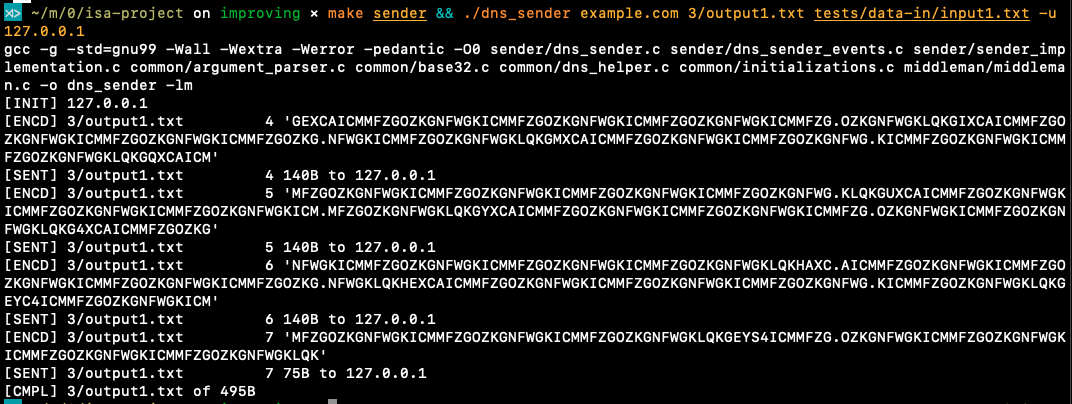
\includegraphics[width=0.77\textwidth]{sender}
    \caption{Ukázka komunikace od klienta}
    \label{fig:a1}
\end{figure}

\begin{figure}[H]
    \centering
    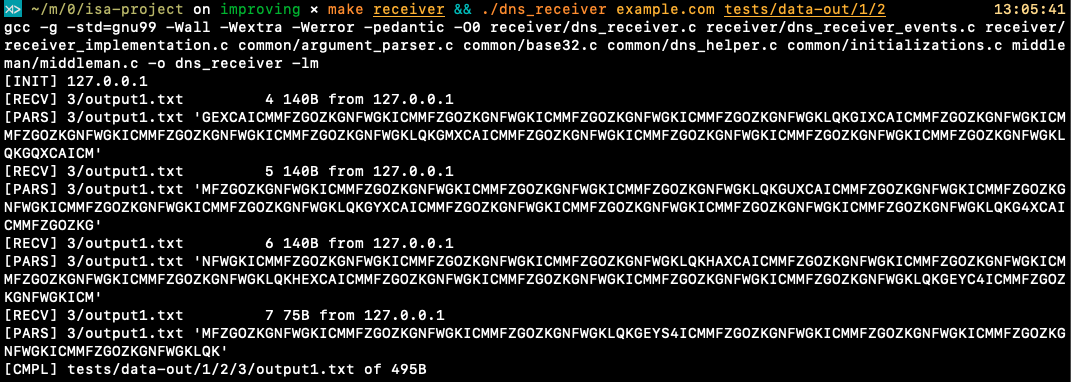
\includegraphics[width=0.77\linewidth]{receiver}
    \caption{Ukázka komunikace od serveru}
    \label{fig:a2}
\end{figure}

\begin{figure}[H]
    \centering
    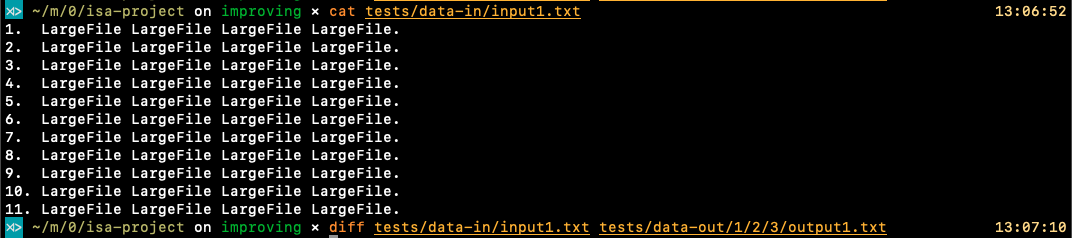
\includegraphics[width=0.77\linewidth]{diff}
    \caption{Ukázka otestovani preneseneho souboru}
    \label{fig:a4}
\end{figure}

\begin{figure}[H]
    \centering
    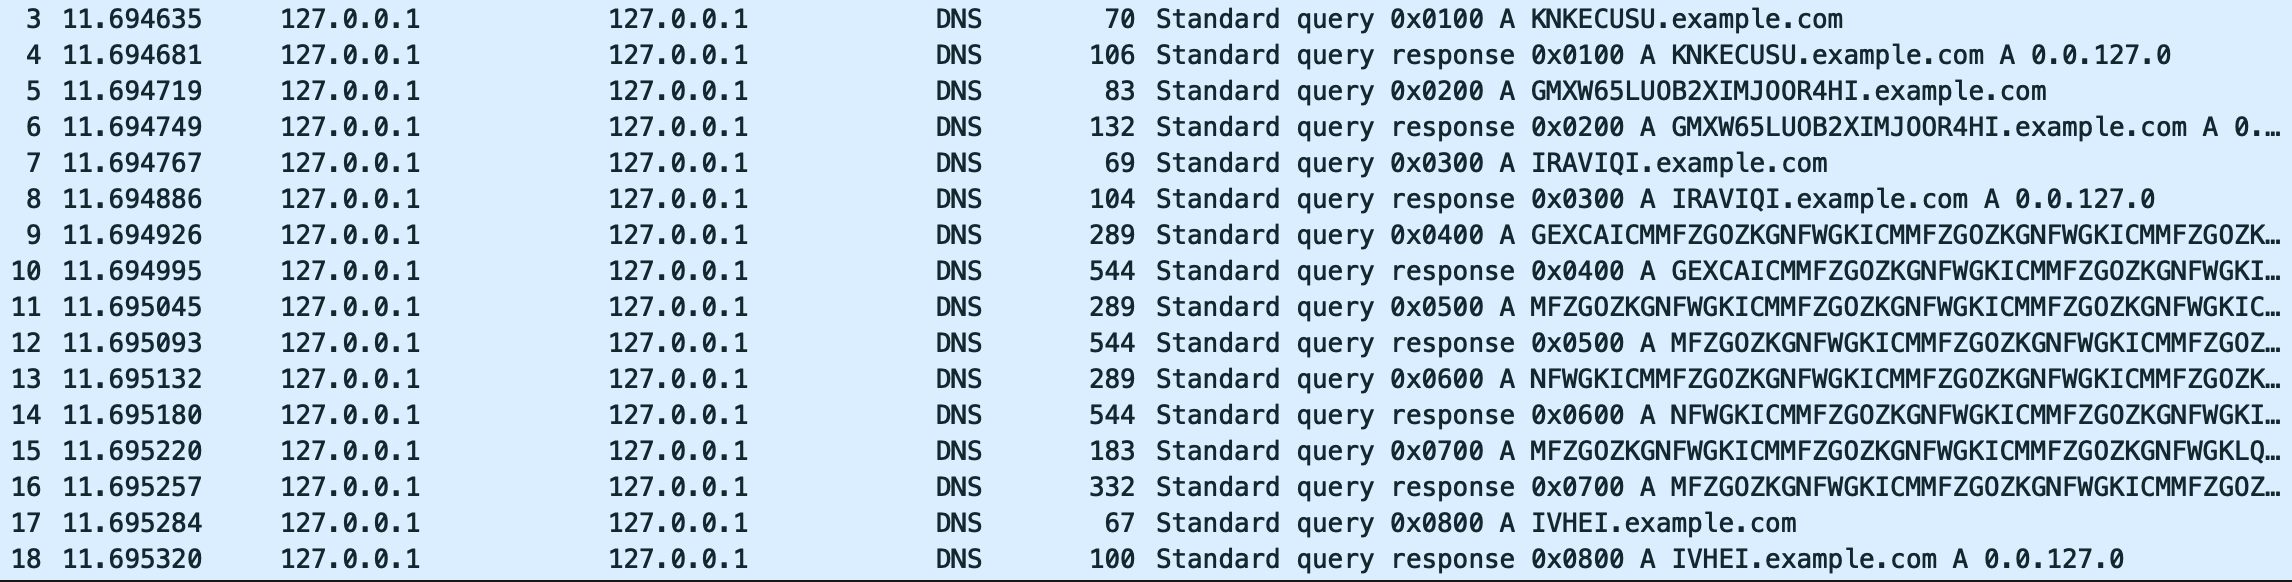
\includegraphics[width=0.77\linewidth]{wireshark}
    \caption{Ukázka komunikace v aplikaci Wireshark}
    \label{fig:a5}
\end{figure}
